% select subfiles base file
\documentclass[TGAI_Laborbericht.tex]{subfiles}
\begin{document}

\chapter{Versuch 4}
\label{chap:VERSUCH_4}

\section{Fragestellung, Messprinzip, Aufbau, Messmittel}
\label{chap:VERSUCH_4_FRAGESTELLUNG}
\subsection{Fragestellung}
Wir untersuchen, was passiert wenn man eine Abtastfrequenz immer weiter der Nyquistfrequenz annähert und über diese hinausgeht.
\subsection{Messprinzip}
Ist wieder der A/D Wandler.
\subsection{Aufbau}
Nun schließen wir einen Sinusgenerator an den Eingang des A/D Wandlers an.
\subsection{Messmittel}
Als Messmittel nutzen wir ein Python Skript, welches uns das Signal und das Spektrum des eingegebenen Signals abbildet.
\section{Messwerte}
\label{chap:VERSUCH_4_MESSWERTE}
Nun stellen wir den Sinusgenerator so ein, dass er eine Frequenz ausgibt, die angefangen bei der halben Nyquist-Frequenz (2000Hz) bis zur doppelten Nyquist-Frequenz (8000Hz) geht.
\section{Auswertung}
\label{chap:VERSUCH_4_AUSWERTUNG}

\begin{figure}[H]
	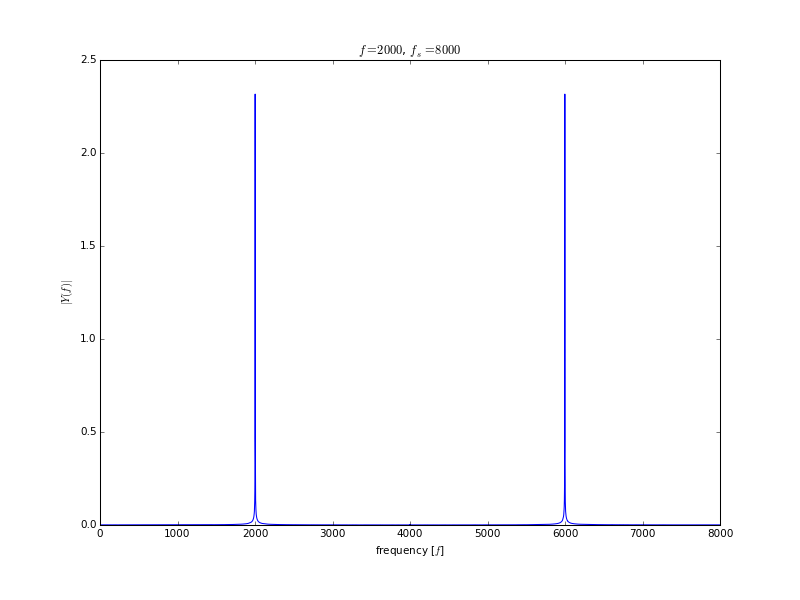
\includegraphics[width=0.7\textwidth]{media/2000-fft.png}
	\label{2000 FFT}
	\caption{2000 FFT}
\end{figure}

\begin{figure}[H]
	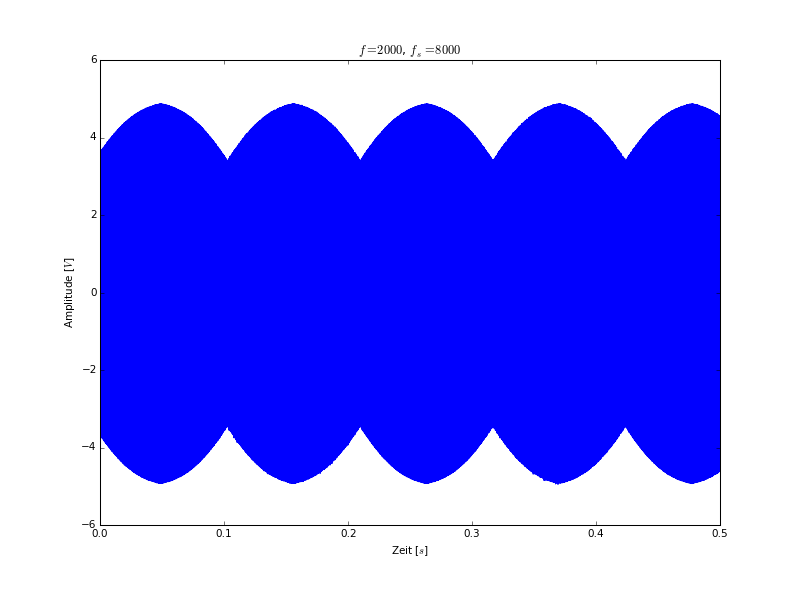
\includegraphics[width=0.7\textwidth]{media/2000-signal.png}
	\label{2000 Signal}
	\caption{2000 Signal}
\end{figure}

\begin{figure}[H]
	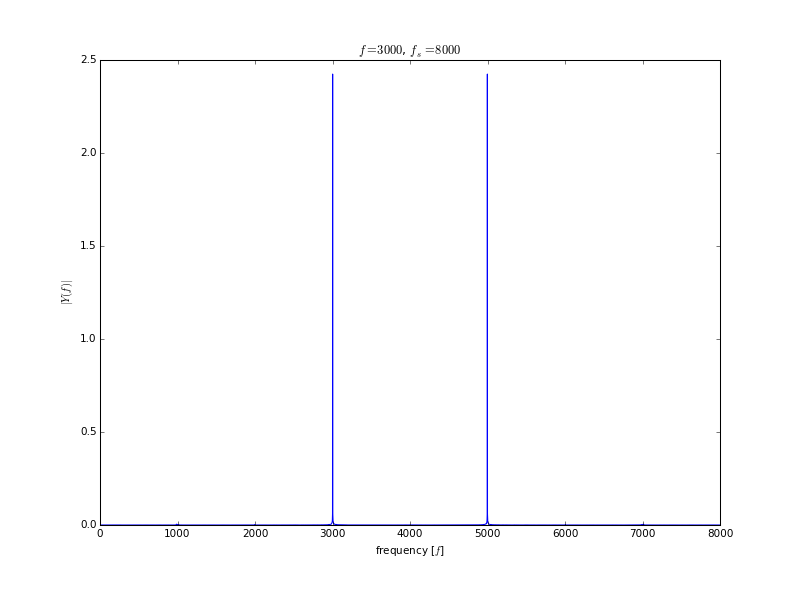
\includegraphics[width=0.7\textwidth]{media/3000-fft.png}
	\label{3000 FFT}
	\caption{3000 FFT}
\end{figure}

\begin{figure}[H]
	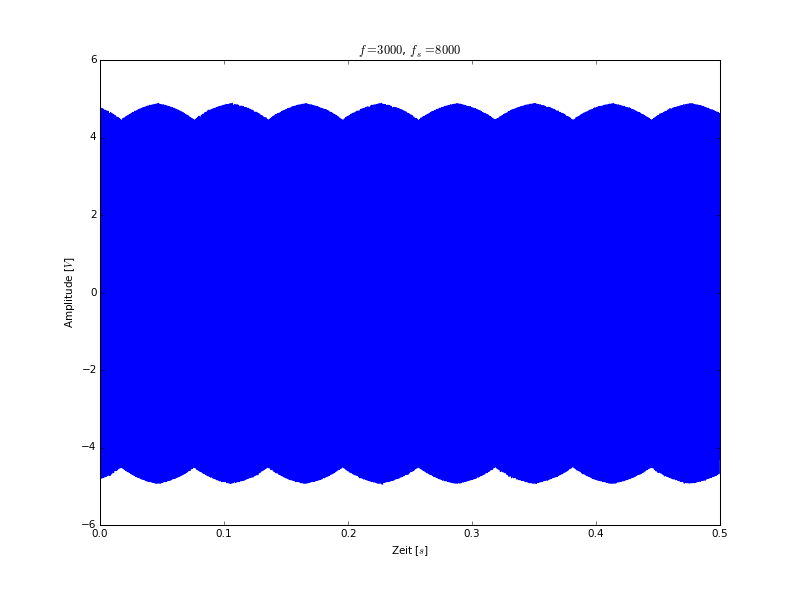
\includegraphics[width=0.7\textwidth]{media/3000-signal.png}
	\label{3000 Signal}
	\caption{3000 Signal}
\end{figure}

\begin{figure}[H]
	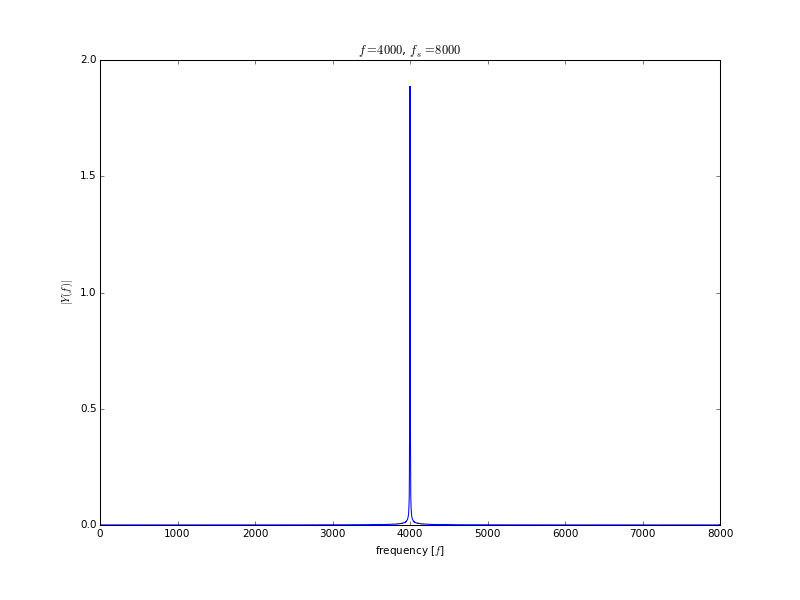
\includegraphics[width=0.7\textwidth]{media/4000-fft.png}
	\label{4000 FFT}
	\caption{4000 FFT}
\end{figure}

\begin{figure}[H]
	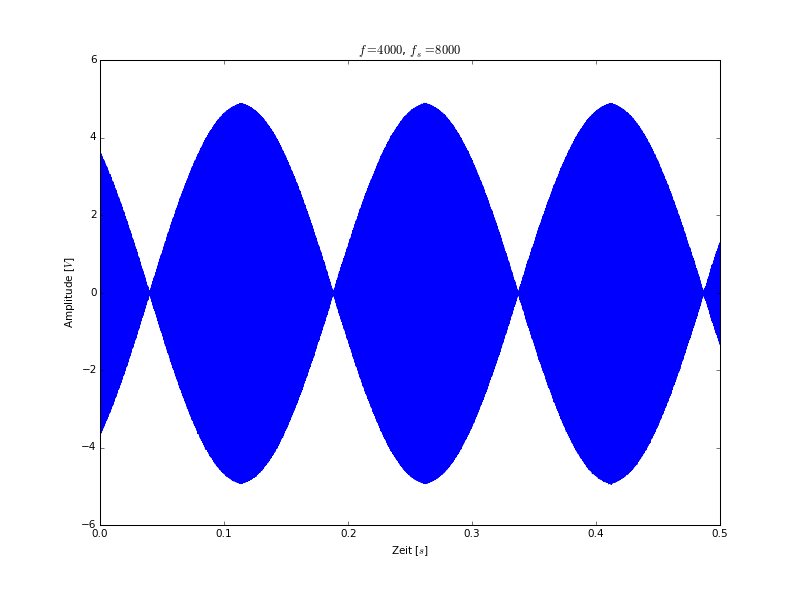
\includegraphics[width=0.7\textwidth]{media/4000-signal.png}
	\label{4000 Signal}
	\caption{4000 Signal}
\end{figure}

\begin{figure}[H]
	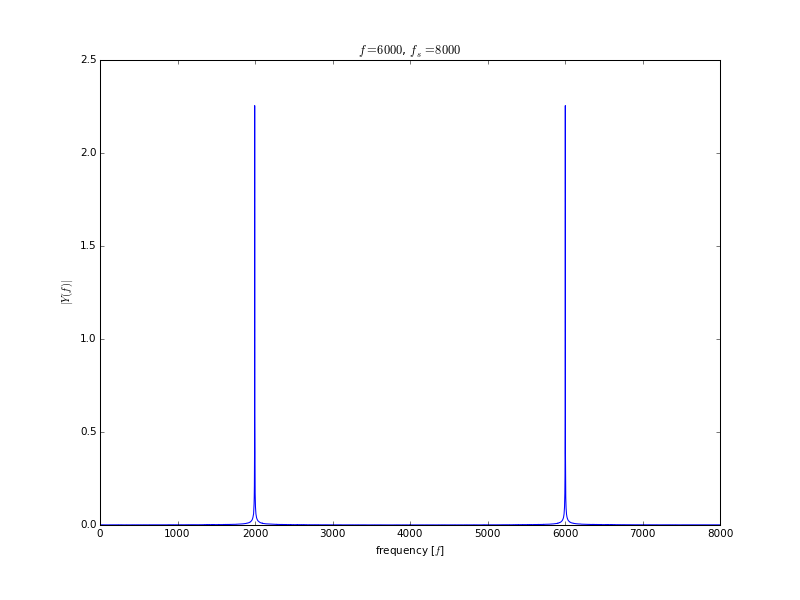
\includegraphics[width=0.7\textwidth]{media/6000-fft.png}
	\label{6000 FFT}
	\caption{6000 FFT}
\end{figure}

\begin{figure}[H]
	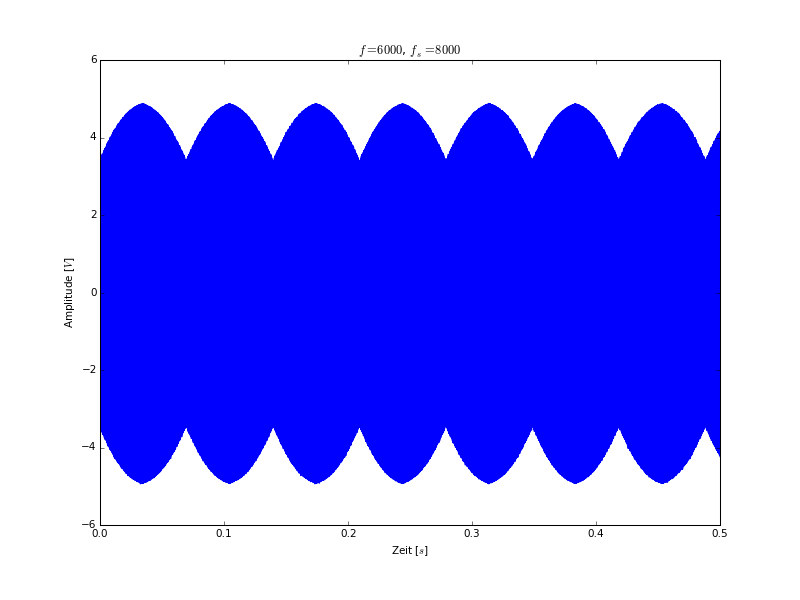
\includegraphics[width=0.7\textwidth]{media/6000-signal.png}
	\label{6000 Signal}
	\caption{6000 Signal}
\end{figure}

\begin{figure}[H]
	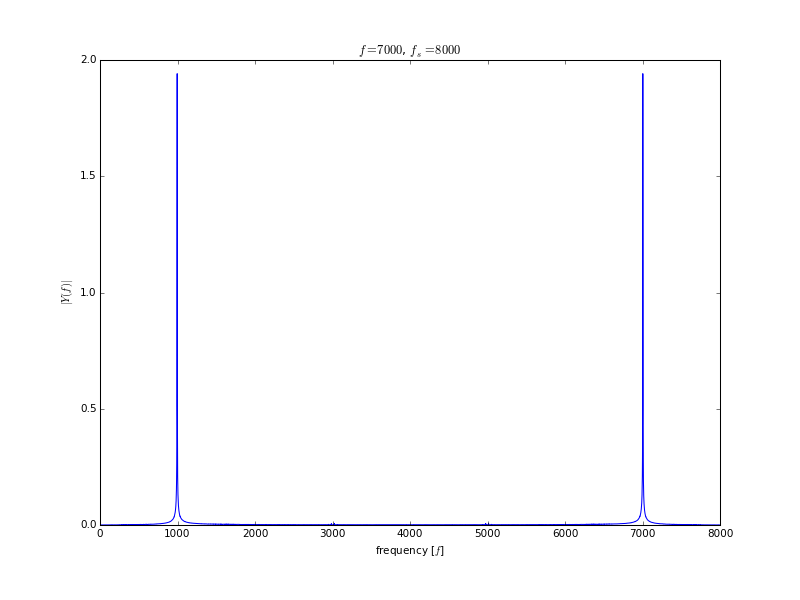
\includegraphics[width=0.7\textwidth]{media/7000-fft.png}
	\label{7000 FFT}
	\caption{7000 FFT}
\end{figure}

\begin{figure}[H]
	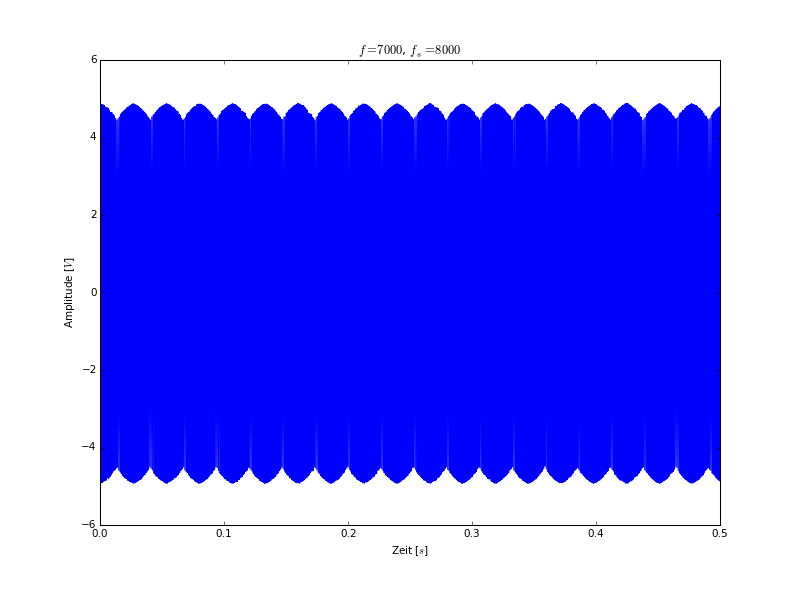
\includegraphics[width=0.7\textwidth]{media/7000-signal.png}
	\label{7000 Signal}
	\caption{7000 Signal}
\end{figure}

\begin{figure}[H]
	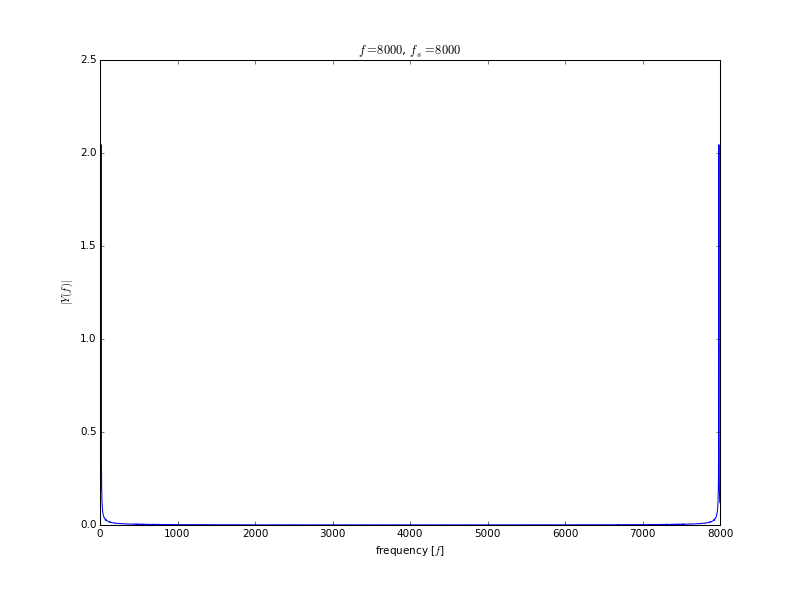
\includegraphics[width=0.7\textwidth]{media/8000-fft.png}
	\label{8000 FFT}
	\caption{8000 FFT}
\end{figure}

\begin{figure}[H]
	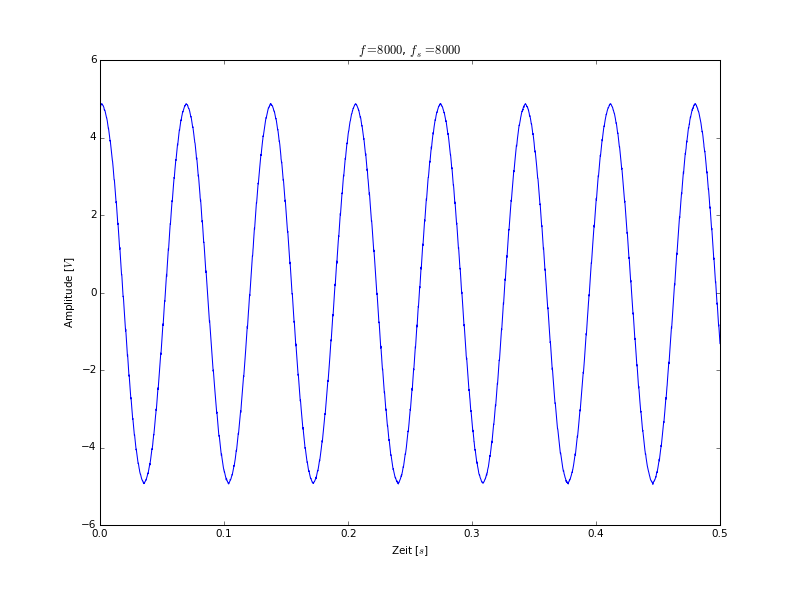
\includegraphics[width=0.7\textwidth]{media/8000-signal.png}
	\label{8000 Signal}
	\caption{8000 Signal}
\end{figure}
\section{Interpretation}
\label{chap:VERSUCH_4_INTERPRETATION}
Die Spektren sind jeweils an der Nyquist-Frequenz achsensymmetrisch. Von 0Hz bis zur Nyquist-Frequenz liegt das eigentliche Spektrum des Signals. Hat man jedoch eine Frequenz die höher ist als die Nyquist-Frequenz, befindet sich diese zwischen Nyquist-Frequenz und 8000. Wenn man die eingegangene Frequenz nicht kennt, würde man also die Falsche Frequenz kriegen, wenn diese über der Nyquist-Frequenz liegt da man in der Regel nur die Seite links der Nyquist-Frequenz betrachtet.

\end{document}